\normalfalse \difficiletrue \tdifficilefalse
\correctionfalse

%\UPSTIidClasse{11} % 11 sup, 12 spé
%\newcommand{\UPSTIidClasse}{12}

\exer{Mouvement RR 3D  $\star\star$ \label{B2:13:07}}
\setcounter{numques}{0}
\UPSTIcompetence[2]{C2-05}
\UPSTIcompetence[2]{B2-13}
\index{Compétence C2-05}
\index{Compétence B2-13}
\index{Mécanisme à 2 rotations 3D}
\ifcorrection
\else
\textbf{Pas de corrigé pour cet exercice.}
\fi

\ifprof
\else
Soit le mécanisme suivant. On a $\vect{AB}=R\vect{i_1}$ et $\vect{BC}=\ell\vect{i_2}+r\vect{j_2}$. On note $R+\ell=L = \SI{20}{mm}$ et $r=\SI{10}{mm}$.
\begin{center}
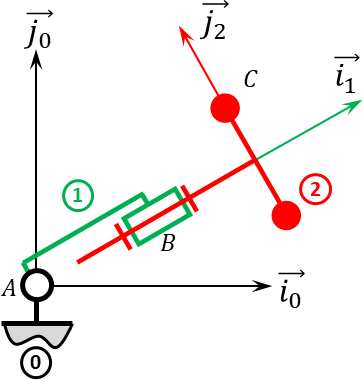
\includegraphics[width=\linewidth]{07_RR3D_01}
\end{center}
\fi

\question{Donner l'ensemble des positions accessibles par le point $B$.}
\ifprof
\else
\fi

\question{Donner l'équation horaire (trajectoire en fonction du temps) du point $B$ dans le mouvement de \textbf{2} par rapport à \textbf{0}.}
\ifprof
\else
\fi






\ifprof
\else
\begin{flushright}
\footnotesize{Corrigé  voir \ref{B2:13:07}.}
\end{flushright}%
\fi